%%% Fiktivní kapitola s ukázkami tabulek, obrázků a kódu

\chapter{Řešítko} \label{resitko}
Abychom mohli dokončit důkaz některých instancí Hypotézy \ref{veta02:hypoteza}, potřebujeme získat požadované stavební bloky. Nabízí se naprogramovat řešítko, které bude umět alespoň některé typy hledaných grafů najít. Hlavním cílem této práce bylo takový program připravit a pomocí něj získat lepší představu o potenciálu uvedené strategie důkazu.

\section{Algoritmus}

Program na vstupu očekává zadání vnější stěny: každý vrchol je zastoupen jedním bitem, který určuje, zda má být ve výsledném grafu stupně 2 nebo 3. Navíc očekává seznam velikostí stěn, které má využít. Na výstupu informuje, zda se mu daný graf podařilo najít (říkejme \textbf{vyplnit}), a umožní jej exportovat.

Postup hledání původně imitoval lidské pokusy o řešení problému: 

\begin{enumerate}
\item nakreslit si vnější stěnu,
\item vybrat si dvojici vrcholů, kterým ještě chybí soused, a spojit je řetízkem vhodné délky (aby nově vzniklá oblast byla stěna a měla velikost z neutrální posloupnosti)
\item krok 2 opakovat, dokud je místo na papíře.
\item Když místo dojde, překreslit si nejvnitřnější, zatím neuzavřenou stěnu (budeme mluvit o \textbf{hranici}). Ta se stane \uv{vnější stěnou} na novém papíře a~pokračovat od~kroku 1.
\item V situaci, kdy nelze dál nic spojit, nebo je jasné, že graf nemůže vyhovovat parametrům, se vrátit podle uvážení zpět.
\end{enumerate}

Výsledek běhu algoritmu je znázorněna na Obrázku \ref{obr03:reseni}.

Kdybychom chtěli znát jen \uv{ano/ne} odpověď, jestli graf existuje, nebylo by vůbec třeba si pamatovat celý rozpracovaný graf, stačilo by pracovat s hranicemi, které navíc stačí reprezentovat jako binární číslo. Výsledkem by pak mohla být jen posloupnost hranic, kterými se prošlo před uzavřením grafu, nebo samotné \uv{ano/ne}. Překvapivě obtížné je pak z této posloupnosti nestrojově získat skutečný graf, proto program nabízí i možnost graf dodatečně rekonstruovat podle prošlých stavů.

V tento okamžik je jasné, že problém je vlastně prohledávání v binárních řetězcích (které reprezentují hranice). Je proto vhodné zmínit, podle jakého kritéria se program rozhoduje, kterým směrem hledat dále. Implementace vždy upřednostňuje ke zpracování již nalezený řetězec nejmenší hodnoty, a pro něj najde všechny další sousedy. Pro názornost přikládáme i pseudokód Vyplň. Vzhledem k návrhu lze algoritmus implementovat vícevláknově -- každou nezpracovanou hranici lze zpracovávat v jiném vlákně, stačí zajistit bezpečnost sdílených datových struktur.

Aby toto prohledávání fungovalo dobře, je třeba trochu zkomplikovat reprezentaci hranice. Hlavním požadavkem bude identita mezi reprezentací (jediným binárním řetězcem) a všemi hranicemi (tedy cykly, na kterých vyznačené vrcholy ještě vyžadují dalšího souseda), které jsou pro algoritmus izomorfní -- tedy všechny rotace a převrácení hranice.


\begin{figure}[h!]\centering
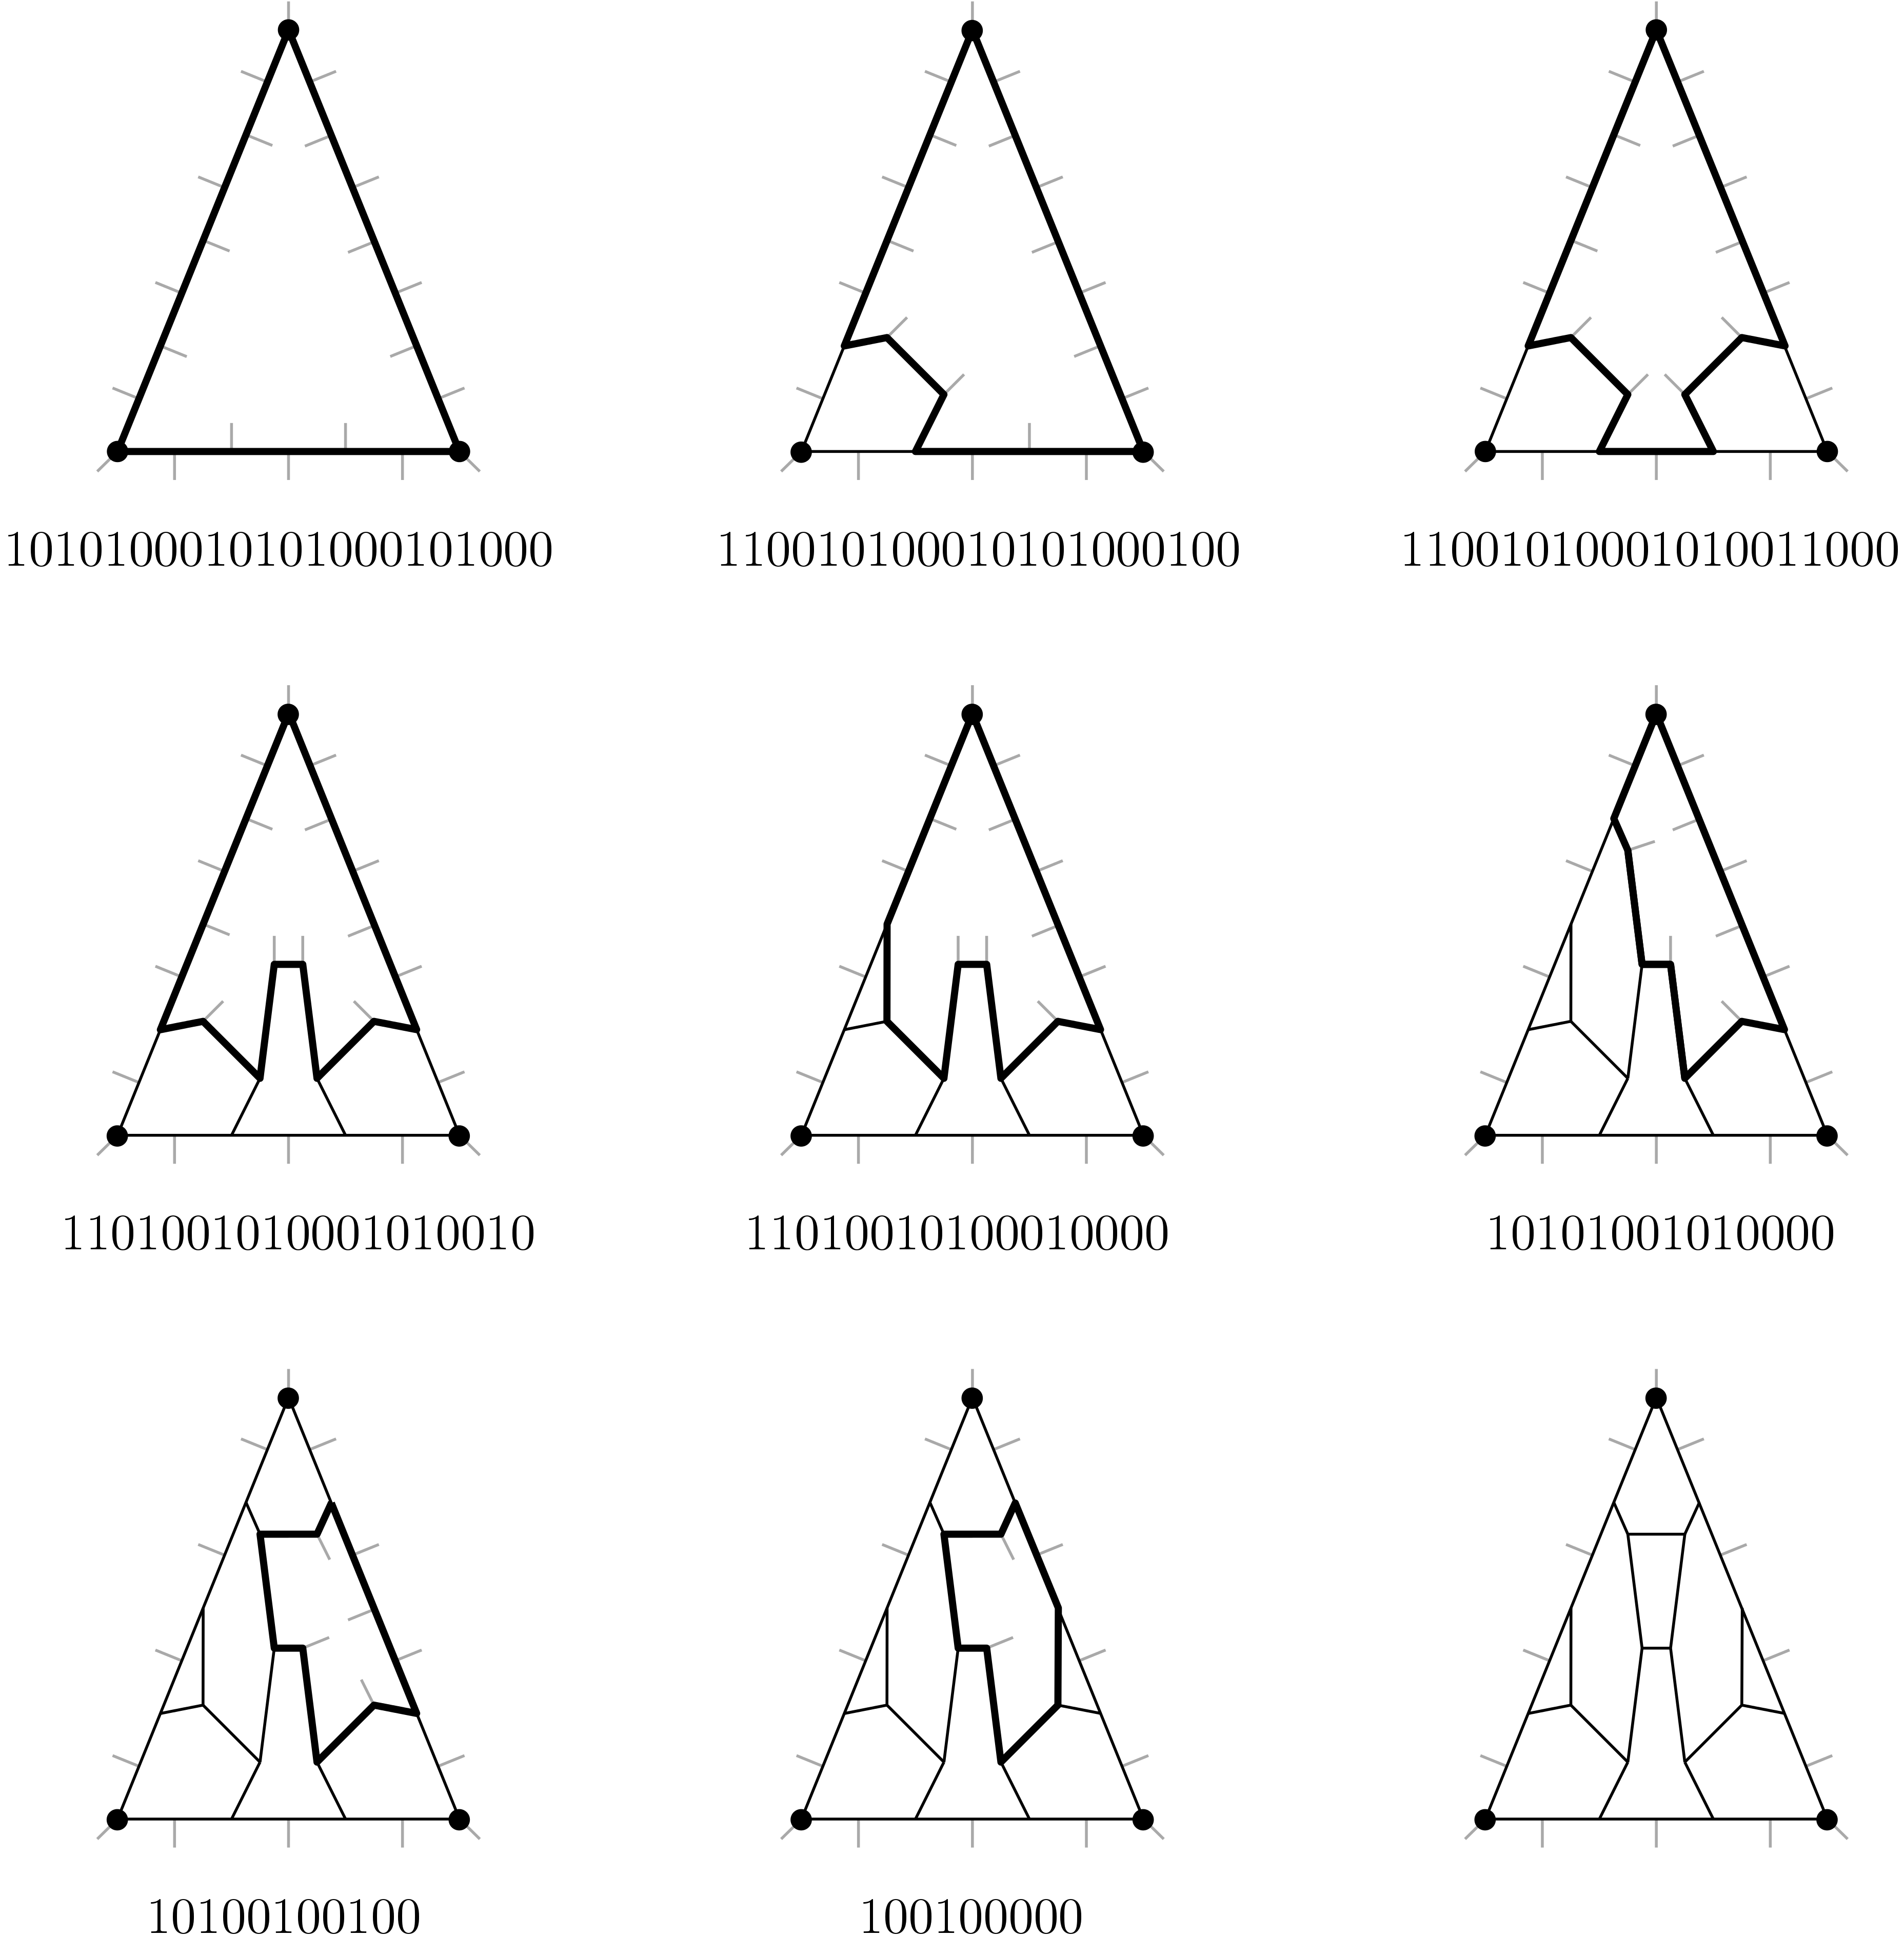
\includegraphics[width=\textwidth]{../img/reseni}
\caption{Možný postup vyplnění (4,4,3)$\lbrace$4,7$\rbrace$-triarku. Hodnota pod grafem vždy odpovídá reprezentaci aktuální, tučně zvýrazněné, hranice.}
\label{obr03:reseni}
\end{figure}

\begin{definice}[Hranice a její reprezentace]\label{def01:1}
Dvojici cyklu $C$ a množiny $I \subseteq V(C)$ nazveme hranicí $H$. Množina $I$ jsou právě ty vrcholy, které ve výsledném vyplnění musí mít dalšího souseda. Pokud  $I = \emptyset$, mluvíme o hranici přímo jako o~stěně a~nedefinujeme pro ni reprezentaci.

Definujme funkci $f(H,(u,v))$ jako charakteristický vektor množiny $I$ následně: každý vrchol H popišme buď znakem 1 (jako I v \uv{in} podle orientace pomyslené hrany) nebo 0 (jako O v \uv{out}). Hodnota $f(H, (u, v))$, kde $H=(C, I)$, $u, v \in V(C)$ a $ \lbrace u, v \rbrace \in E(C)$, se pak získá zaznamenáním popisků vrcholů $H$, začínaje vrcholem $u$, pokračujíce vrcholem $v$ a dále po hranách $C$. 

Reprezentací hranice je hodnota $\max_{\lbrace u, v \rbrace \in E(C)} {f(H,(u,v))}$.
\end{definice}

Objasněme pojem opět jednoduchým pozorováním a Obrázkem \ref{obr03:reseni} -- posloupností hranic s jejich reprezentacemi, která řeší (4,4,3)$\lbrace$4,7$\rbrace$-triark. 


\begin{tvrz}
Při výpočtu reprezentace podle definice hledáme maximum přes $2 |V(C)|$ hodnot a reprezentace každé hranice začíná znakem 1.
\end{tvrz}

\begin{dukaz}
Každý vrchol v C má dva sousedy, tedy v (multi)množině, ze které hledáme řetězce je $2 |V(C)|$ (ne nutně různých) hodnot. Odpovídá to představě, že zkoušíme začít v každém vrcholu a čteme v obou směrech. Vzhledem k tomu, že $I\neq \emptyset$, je v každém přečteném řetězci alespoň jedna jednička. Hledání maxima zajistí, že se upřednostní řetězec, který jedničkou začíná (ten je dostupný, protože se začínalo číst i z vrcholů, které jsou v $I$).  
\end{dukaz}

\makeatletter
\algrenewcommand\ALG@beginalgorithmic{\footnotesize}
\makeatother


\begin{algorithm}
\label{alg:Vypln}
\begin{algorithmic}
\Procedure{Vyplň}{reprezentace vnější hranice \textit{vnějšíHraniceStdRep}, velikosti povolených stran \textit{stěny}, \textit{limit}}

\State \textit{nevyřešenéHranice} $\gets$ \textit{vnějšíHraniceStdRep}	
\State \textit{přechody} $\gets \emptyset$ 		
 \While {\textit{přechody}.Počet $\leq$ \textit{limit} \textbf{AND} \textit{nevyřešenéHranice}.Počet $\neq 0$ }
 \State \textit{hranice} $\gets$ \textit{nevyřešené}.Nejmenší
\State \textit{rotace} $\gets$ \textbf{RotaceHraniceZačínajícíInVrcholem}(\textit{hranice})
\ForAll { \textit{h} in \textit{rotace}}
\ForAll {\textit{s} in \textit{stěny}}
\State	\textit{nováHraniceStdRep} $\gets$ \textbf{ZkusSpojitPrvníDvaInVrcholy}(\textit{h, s}) 	
	\If {\textit{nováHraniceStdRep}.MáHodnotu}  
\State		\textit{nevyřešenéHranice}.Přidej(\textit{nováHraniceStdRep})
\State		\textit{přechody}.Přidej(\textit{nováHraniceStdRep, hranice})
\EndIf
	\If {\textbf{JeStěna}(\textit{nováHraniceStdRep, stěny})} 
\State		vrať \textbf{Cesta}(\textit{přechody, nováHraniceStdRep, vnějšíHraniceStdRep})
\EndIf

\EndFor
\EndFor
\EndWhile
\State oznam nenalezení
\EndProcedure

\end{algorithmic}
\end{algorithm}


Pro jistotu poznamenejme, že pokud program hledaný graf nenašel, může, ale nemusí to znamenat, že neexistuje.


\bigskip

Podle předchozí kapitoly pro dokončení důkazu pro konkrétní dvojici $p$ a~$q$ a~nějaké přirozené $k$ potřebujeme tyto čtyři typy grafů:
\begin{description}
\item[(i)] ($k$, $k$, $k$)$Q$-triark;
\item[(ii)] ($k$, $k$, $k-1$)$Q$-triark;
\item[(iii)] ($mk$, $mk$, $x$)$Q\cup \lbrace l\rbrace$-triark, kde je právě jedna stěna velikosti $l$;
\item[(iv)] prstenec, který dokáže spojit dva stejně velké, rovnostranné triarky.
\end{description}

Pro dané $k$ získáme grafy (i) a (ii) z řešítka hned. Pro zbylé je nutné pomoci si konstrukcí, která se ukázala jako úspěšná pro některé neutrální posloupnosti. O~výsledcích získaných z programu píšeme v Kapitole \ref{vysledky}.

\begin{figure}[h]\centering
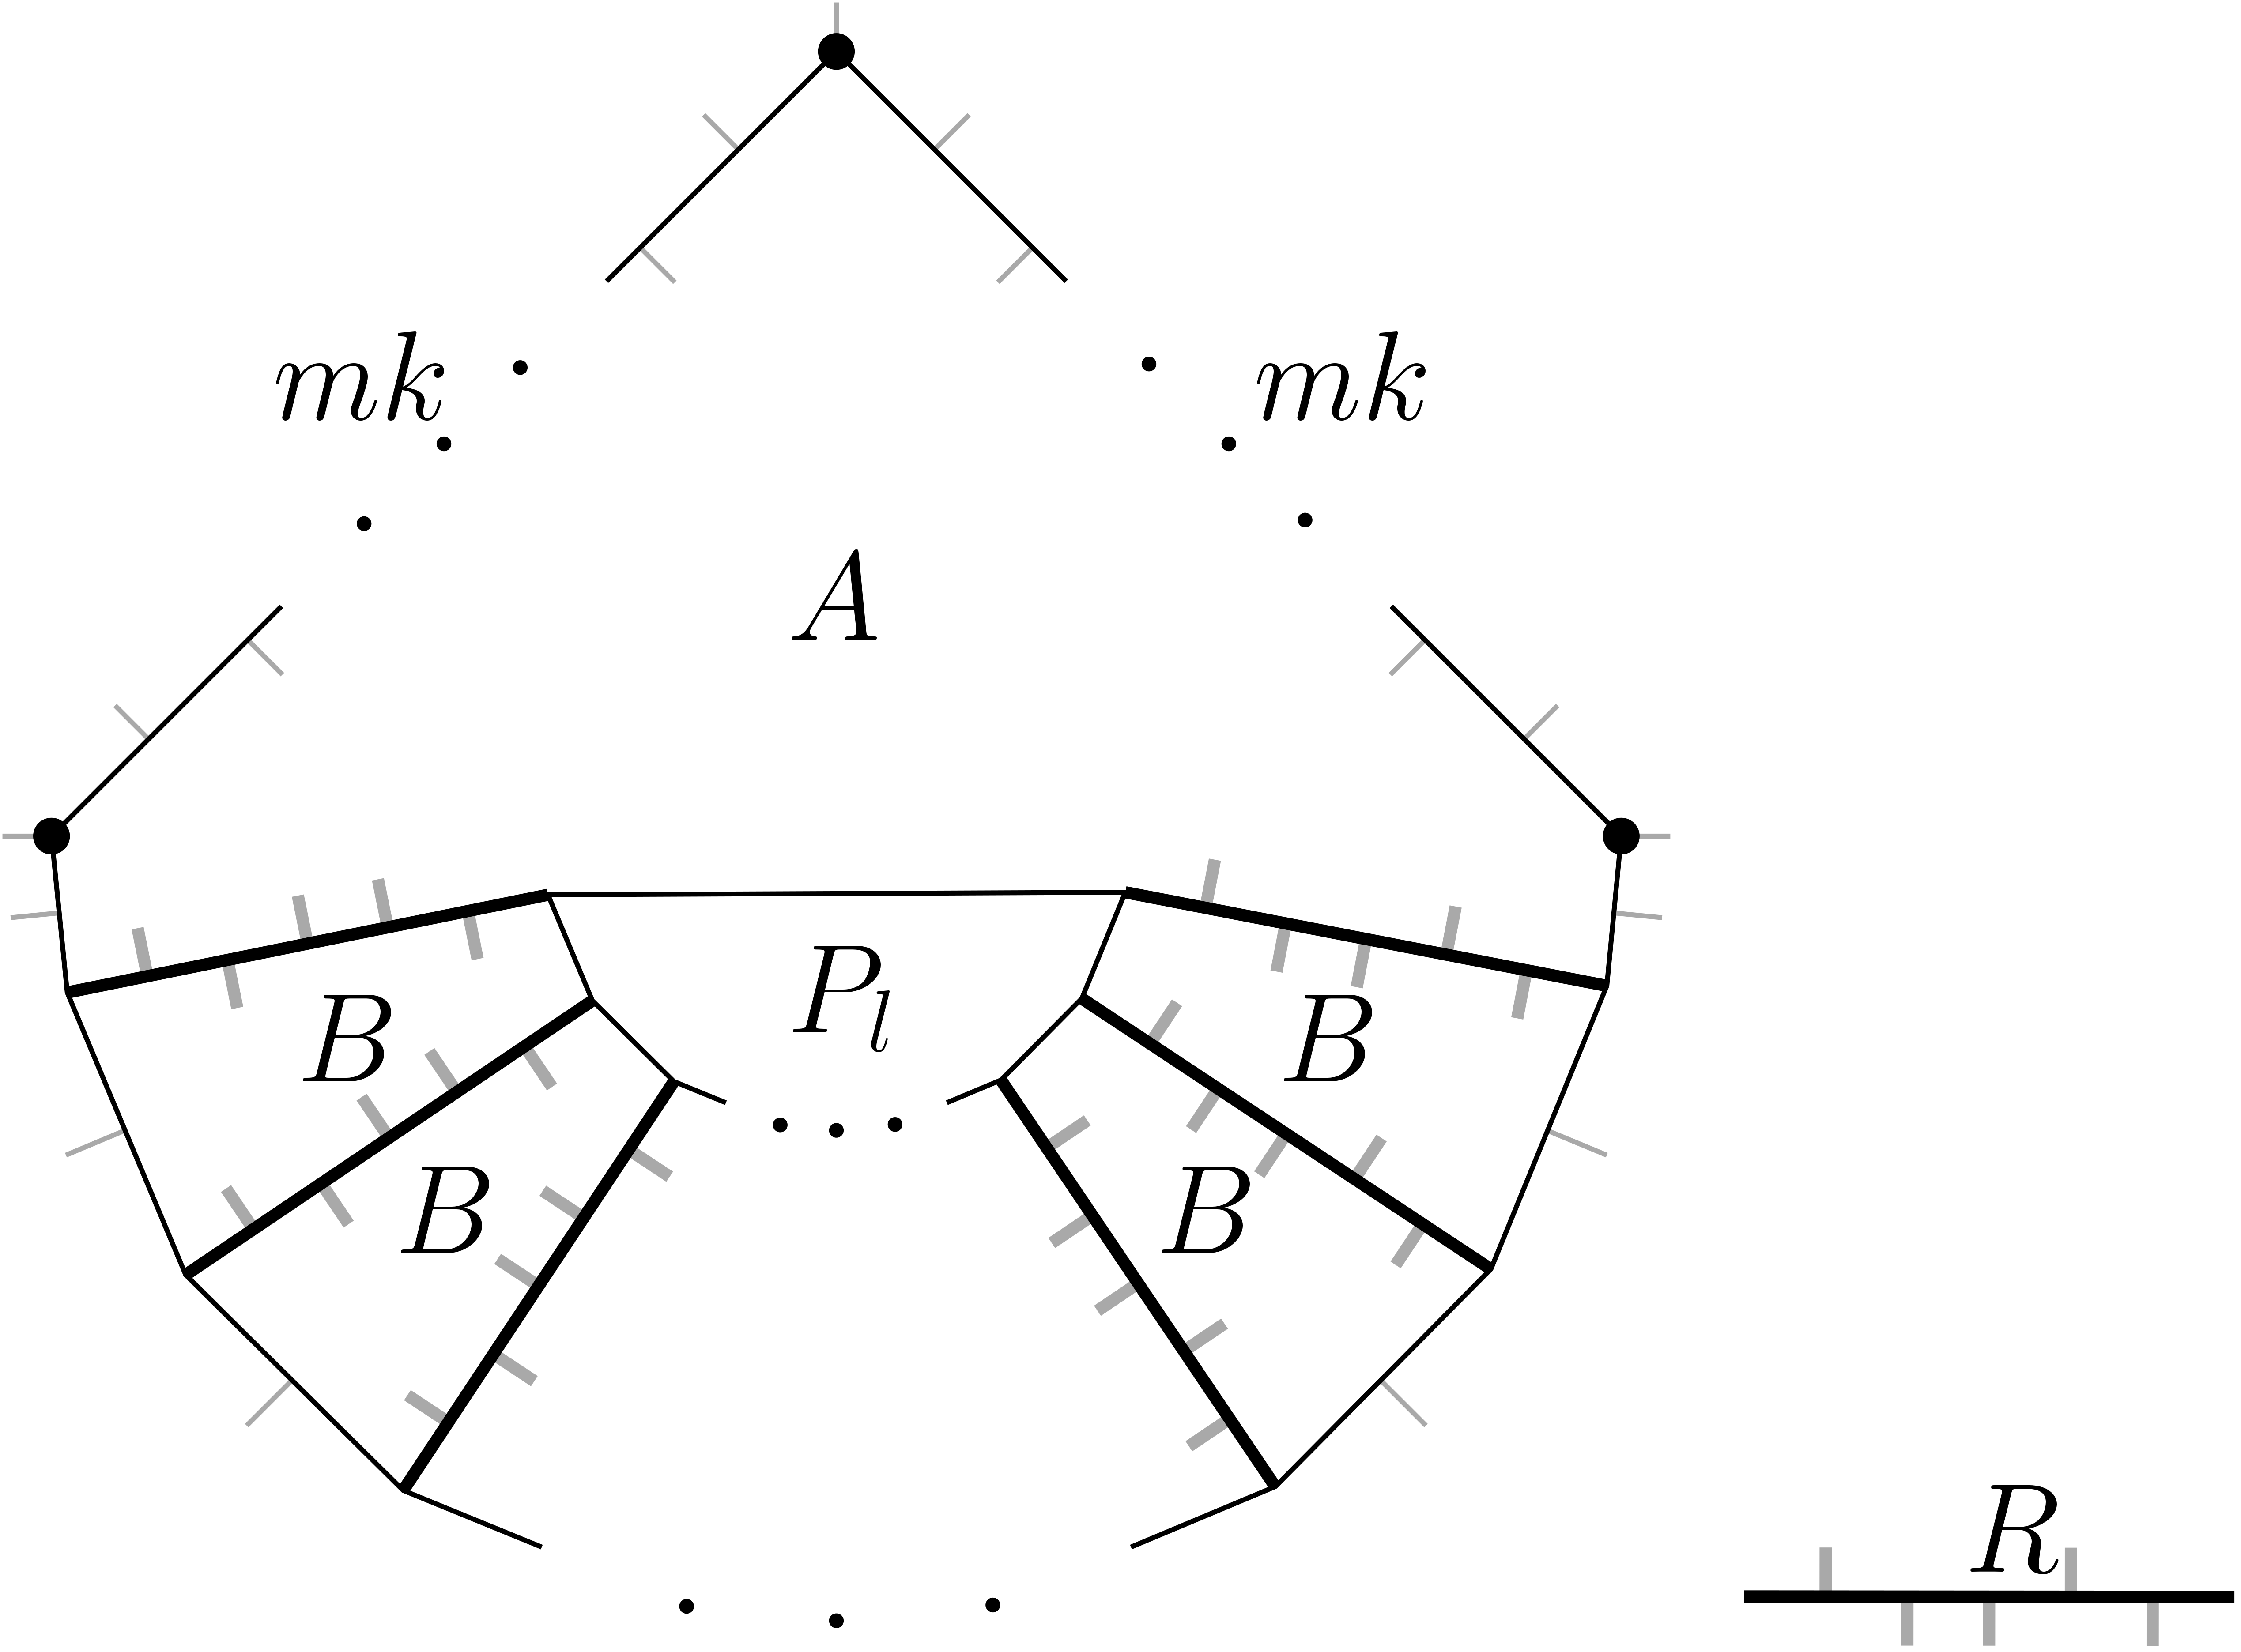
\includegraphics[width = 80mm]{../img/iii-construction}
\caption{Konstrukce grafu typu (iii) pomocí řetízků $R$, konkrétně ($mk$, $mk$, $l+1$)-triarku s $l$-úhelníkem $P_l$ jako jádro.}
\label{obr03:konstrukceiii}
\end{figure}

Na graf (iii) se neumíme zeptat přímo, protože potřebujeme v grafu mít právě jednu stěnu délky $p_l$. Spojme proto stěnu s vnější stěnou triarku ručně a ptejme se na výplň vzniklých oblastí $A$ a $B$. Ke spojení použijeme $l$ kopií řetízku $R$, každý napojíme na jeden z vrcholů jádra a druhé konce spojíme s \uv{in} vrcholy základny triarku. V řetízku navíc fixujeme, na které straně od něj budou mít které jeho vrcholy třetího souseda (znázorněno šedě v Obrázku \ref{obr03:konstrukceiii}). Konstrukce je obecná pro všechny přípustné hodnoty $l$, tedy není závislá na volbě $p$. Nevíme ani o důvodu, který by implikoval nemožnost jejího využití pro libovolné $q$.


Podobnou konstrukci tvoříme i pro graf typu (iv). V tomto případě za pomoci řetízků spojujeme odpovídající vrcholy rovnostranných, stejně velkých triarků $T_1$ a $T_2$. Vzniknou dva typy oblastí -- $C$ při rozích triarku a $D$ mezi odpovídajícími úseky stran triarků. Přesný nákres je na Obrázku \ref{obr03:konstrukceiv}. Poznamenejme, že pokud jde graf nakreslit na povrch hranolu, je rovinný. 

\begin{figure}[h]\centering
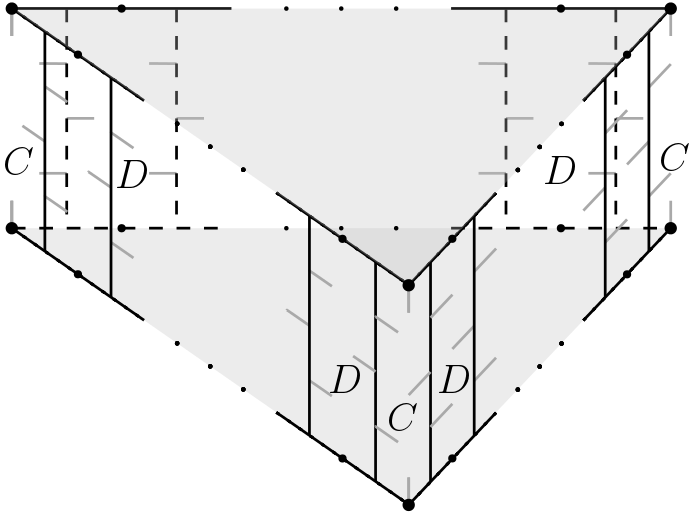
\includegraphics[width = 60mm]{../img/iv-construction}
\caption{Konstrukce grafu typu (iv), slepované triarky jsou vyznačené šedě, prstenec odpovídá plášti.}
\label{obr03:konstrukceiv}
\end{figure}

Tyto konstrukce jsou v řešítku implementovány, pro ukázku přikládáme pseudokód Dokaž. Výslednému program stačí zadat seznam velikostí stěn, které mohou tvořit neutrální posloupnost. Pokud pro daný seznam stěn existuje více neutrálních posloupností, využije program pro~každý pomocný graf libovolnou z~nich.


\begin{algorithm}
\label{alg:dokaz}
\begin{algorithmic}
\Procedure{Dokaž}{velikosti povolených stran \textit{stěny}, \textit{limit}}
\State \textit{řetízky} \Comment{Předdefinovaná množina řetízků}
\State \textit{velikostiStran} \Comment{Předdefinovaná množina velikostí stran}
\State 
\State \textit{iGraf} $\gets$ \textit{velikostiStran}.Kde(\textit{k} $\Rightarrow$ \textbf{JdeVyplnit}(\textbf{HraniceTriarku}(\textit{k, k, k}), \textit{stěny, limit}))
\State \textit{iiGraf} $\gets$ \textit{iGraf}.Kde(\textit{k} $\Rightarrow$ \textbf{JdeVyplnit}(\textbf{HraniceTriarku}(\textit{k, k, k-1}), \textit{stěny, limit}))
\State \textit{řetízkyA} $\gets$ \textit{řetízky}.Kde(\textit{r} $\Rightarrow$ \textit{iiGraf}.Existuje(\textit{k} $\Rightarrow$ \textbf{JdeVyplnit}(\textbf{HraniceA}(\textit{r, k}), \textit{stěny}, \textit{limit})
\State \textit{iiiGraf} $\gets$ \textit{řetízkyA}.Kde(\textit{r} $\Rightarrow$ \textbf{JdeVyplnit}(\textbf{HraniceB}(\textit{r}), \textit{stěny}, \textit{limit}))
\State \textit{řetízkyC} $\gets$ \textit{řetízky}.Kde(\textit{r} $\Rightarrow$ \textbf{JdeVyplnit}(\textbf{HraniceC}(\textit{r}), \textit{stěny}, \textit{limit}))
\State \textit{ivGraf} $\gets$ \textit{řetízkyC}.Kde(\textit{r} $\Rightarrow$ \textbf{JdeVyplnit}(\textbf{HraniceD}(\textit{r}), \textit{stěny}, \textit{limit}))
\State 
\State vrať \textit{iiiGraf}.Počet $ \neq 0$ \textbf{AND} \textit{ivGraf}.Počet $\neq 0$

\EndProcedure

\end{algorithmic}
\end{algorithm}
%\newpage 


\section{Program a výstupy} \label{prg&vystupy}

Implementaci výše popsaného algoritmu k práci přikládáme, Příloha \ref{priloha:aplikace}, jako spustitelný program (pro Windows) i zdrojové kódy. Jde o standardní konzolovou aplikaci, včetně nápovědy pro použití v podobě \texttt{-h} argumentu při spuštění. Například Příloha \ref{priloha:vysledky} včetně dat pro Tabulku \ref{obr03:tabvysledkycele} lze vygenerovat argumenty \texttt{-r -l 100000 -{}-ExportAsAll}.

Zastavme se u typů souborů, které program může generovat:
\begin{description}

\item[Graf] vypíše nalezený graf jako seznam hran.
\item[Hranice] vypíše posloupnost hranic, podle kterých je graf sestaven, příkladem může být Obrázek \ref{obr03:reseni}.
\item[Stěny] vypíše vnitřní stěny grafu, které odpovídají chodu algoritmu a které jinak nemusí být dány jednoznačně.
\item[Graphviz -- neato] vypíše graf v jazyku DOT, navíc rozmístí vrcholy vnější hranice grafu na kružnici.
\item[Tuttovo kreslení] vypíše skript pro SageMath, který graf vykreslí podle barycentrické metody, je v něm připravená funkce pro změnu vah vrcholů.

\end{description}


